\documentclass{article}

\usepackage[final,main]{neurips_2025}

\usepackage[utf8]{inputenc}
\usepackage[T1]{fontenc}
\usepackage{hyperref}
\usepackage{url}
\usepackage{booktabs}
\usepackage{amsfonts}
\usepackage{nicefrac}
\usepackage{microtype}
\usepackage{xcolor}
\usepackage{amsmath}
\usepackage{amssymb}
\usepackage{graphicx}
\usepackage{subcaption}
\usepackage{threeparttable}
\usepackage{array}
\usepackage{placeins}

\captionsetup{font=small,skip=2pt}
\setlength{\textfloatsep}{5pt plus 2pt minus 2pt}
\setlength{\floatsep}{4pt plus 2pt minus 2pt}
\setlength{\intextsep}{4pt plus 2pt minus 2pt}

\title{NeuroCLIP + LATA:\\
Action Semantics and Latency-Aware Alignment for EEG-to-Video Decoding}

\author{
Rachel Li \\
\texttt{lirachel@mit.edu}
\and
Emma Wang \\
\texttt{ewang13@mit.edu}
\and
Winston Qian \\
\texttt{winstonq@mit.edu}
}

\begin{document}

\maketitle

\vspace{-0.5em}
\begin{center}
\small
\begin{tabular}{ll}
\textbf{Winston's Repo:} & \url{https://github.com/winstonqian/mmai} \\
\textbf{Emma's Repo:} & \url{https://github.com/greenMangoes13/mmai} \\
\textbf{Rachel's Repo:} & \url{https://github.com/hnxnq7/mmai} \\
\end{tabular}
\end{center}
\vspace{-0.8em}

% ============================================================
\section*{Abstract}
% ============================================================

Decoding natural video perception from non-invasive electroencephalography (EEG)
is an important step toward practical brain--computer interfaces, but current
EEG-to-video benchmarks leave two questions underexplored: which visual concepts
are most reliably represented in EEG, and when does the corresponding neural
evidence emerge after stimulus onset? We study these questions on SEED-DV, a
40-concept natural video EEG benchmark, through two complementary contributions.
First, we introduce \textbf{NeuroCLIP}, a
CLIP-aligned EEG retrieval probe that maps EEG into a frozen semantic vision-language
space and evaluates concept-level decodability through 40-way retrieval. NeuroCLIP
achieves 4.60\% Recall@1 and 17.47\% Recall@5 on concept retrieval, exceeding
chance (2.5\% / 12.5\%) and matching the scale of supervised EEG2Video-style
classification baselines (4.37\% top-1, 17.17\% top-5). More importantly, it
turns aggregate performance into an error-analysis tool: CLIP embedding isolation
does not predict EEG decodability ($r{=}0.036$, $p{=}0.827$), while action-rich
concepts such as sports, music, and people are substantially more decodable than
passive scenes (6.8\% vs.\ 3.8\%, $p{<}10^{-7}$). Second, we propose
\textbf{LATA}, a latency-aware temporal alignment module that learns a soft
distribution over biological neural delays during EEG--video contrastive training.
On all 20 SEED-DV subjects, LATA recovers a consistent nonzero delay preference:
14/20 subjects peak at a two-chunk lag, 6/20 peak at a one-chunk lag, and no
subject peaks at zero lag, with mean expected delay $1.58 \pm 0.05$ chunks
($\approx$790\,ms). These results indicate that progress on EEG-to-video decoding
requires attention to both stimulus semantics and neural response latency, not
only decoder architecture.

% ============================================================
\section{Introduction}
% ============================================================

Decoding visual experience from brain activity is a long-standing goal in
multimodal AI and brain--computer interfaces (BCIs). If a model can infer what a person is
seeing from neural activity alone, it can support assistive communication,
closed-loop rehabilitation, and scientific analysis of visual processing.
Functional MRI has enabled impressive static image and video reconstruction
because it captures spatially detailed cortical activity, but it is expensive,
immobile, and temporally slow~\citep{takagi2023highres,chen2023cinematic}.
Electroencephalography (EEG), by contrast, is non-invasive, portable, and
temporally precise, making it a realistic sensing modality for deployable BCIs.
The difficulty is that EEG is noisy, subject-specific, spatially coarse, and
delayed relative to the stimulus that caused it.

Recent work shows that EEG contains decodable visual information. EEG2Video
introduced the SEED-DV dataset and demonstrated that 62-channel EEG can support
concept, color, and motion decoding from short natural video clips~\citep{liu2024eeg2video}.
Following work has used diffusion models, video priors, and multimodal embedding
spaces to improve brain-to-vision generation~\citep{li2024visual,dynamind2025,zhou2026mindcine}.
However, a single aggregate classification score does not reveal what the EEG
signal actually represents. A model may do well on some concepts and fail on
others for reasons that have little to do with the visual embedding geometry used
by the decoder. In addition, most EEG-video alignment methods treat EEG and video
as synchronous streams. This assumption is biologically wrong: visual responses
arrive after a latency, with early sensory components around 100\,ms and later
semantic components several hundred milliseconds after stimulus onset~\citep{luck2014erp}.
\begin{figure}
    \centering
    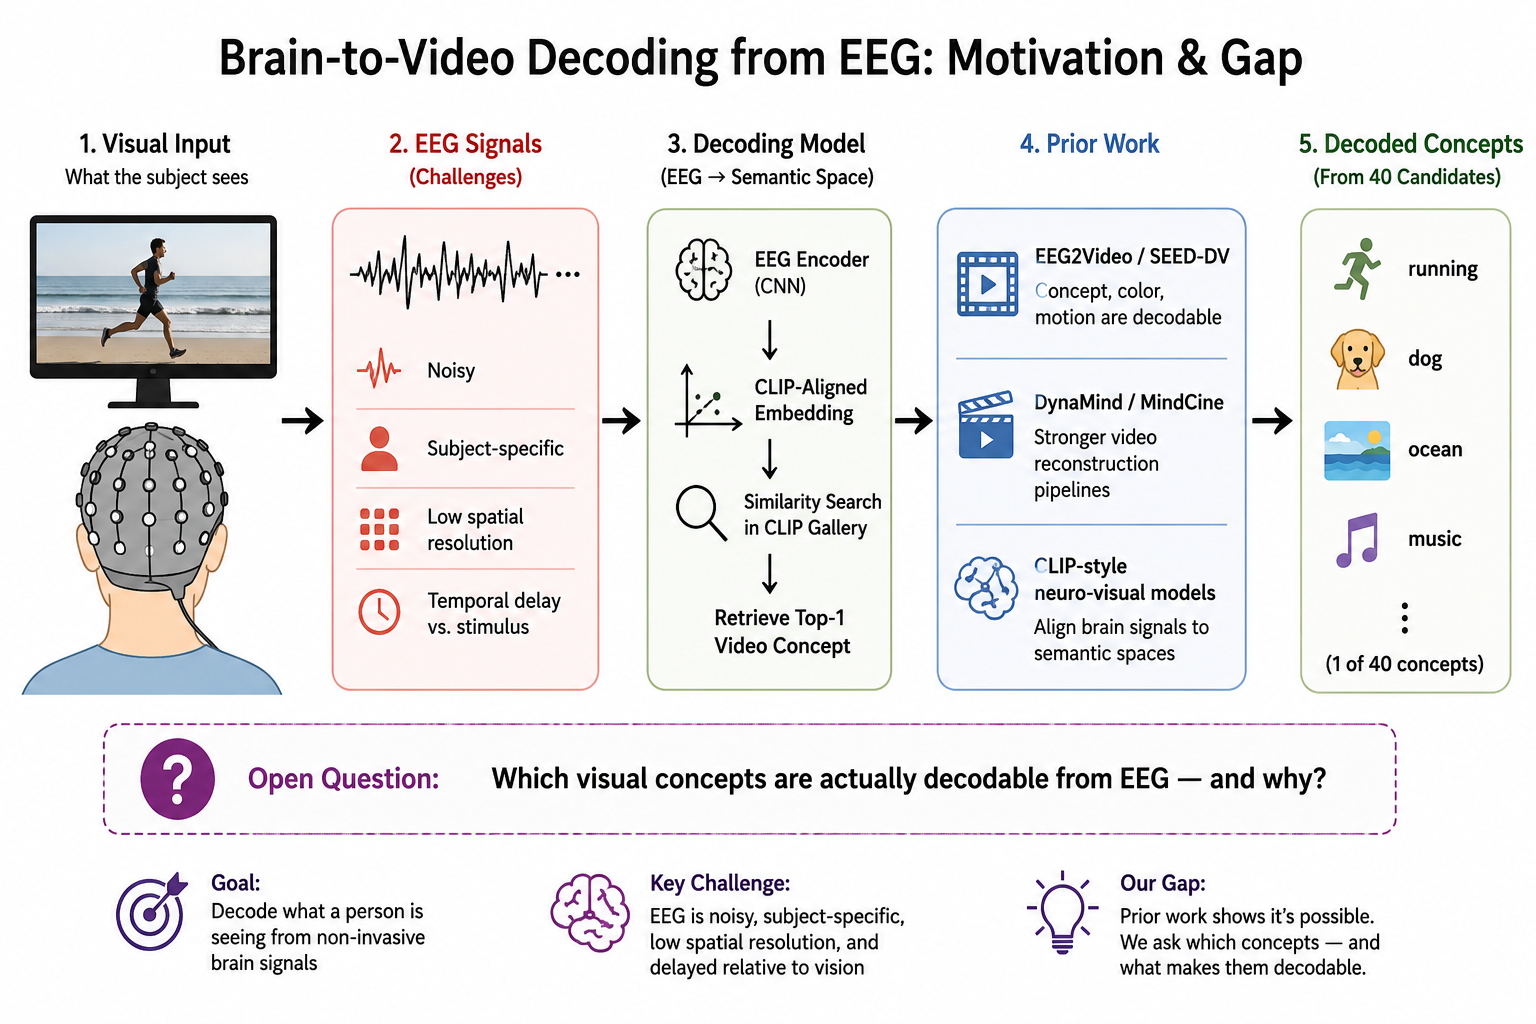
\includegraphics[width=0.9\linewidth]{motivation.png}
\caption{Brain-to-Video Decoding from EEG: Motivation and Gap. A subject views a video clip, 62-channel EEG is encoded into a CLIP-aligned embedding, and the closest concept is retrieved from 40 candidates. Prior work establishes that decoding is possible but reports only aggregate scores. We ask which concepts are decodable and why — and when the neural evidence arrives.}
    \label{fig:placeholder}
\end{figure}

In this paper, we address both questions through two contributions. NeuroCLIP is a lightweight CLIP-aligned EEG retrieval probe that maps EEG features into a frozen CLIP concept gallery and evaluates per-concept retrieval, turning CLIP from a generative backbone into an analysis instrument that tests whether decodability follows CLIP geometry, semantic category, or protocol artifacts. LATA (Latency-Aware Temporal Alignment) is a differentiable alignment module that learns a soft distribution over candidate neural delays during EEG–video contrastive training, recovering response latency without supervision. Together, NeuroCLIP characterizes which concepts are represented in EEG, and LATA estimates when the corresponding neural evidence arrives. We evaluate both on SEED-DV under leave-one-block-out within-subject cross-validation, with audits for normalization leakage and run-position artifacts. 

% ============================================================
\section{Related Work}
% ============================================================

\paragraph{Brain-to-vision decoding.}
Early visual decoding work focused on fMRI because of its high spatial
resolution. Recent systems reconstruct images from fMRI using latent diffusion
priors~\citep{takagi2023highres,ozcelik2023natural} and extend reconstruction to
naturalistic video~\citep{chen2023cinematic}. EEG-based visual decoding is more
challenging, but its temporal resolution and portability are valuable.
Li et al.~\citep{li2024visual} decode visual experience from EEG using guided
diffusion, while EEG2Video introduces SEED-DV and shows that concept, color, and
motion attributes are decodable from 62-channel EEG~\citep{liu2024eeg2video}.
DynaMind~\citep{dynamind2025} and MindCine~\citep{zhou2026mindcine} further
study dynamic visual decoding, temporal consistency, and data efficiency. Our
work differs by emphasizing semantic and temporal diagnostics rather than
photorealistic reconstruction quality alone.

\paragraph{Contrastive multimodal alignment.}
Contrastive learning has become a standard way to align modalities into shared
embedding spaces. CLIP aligns image and text representations using large-scale
contrastive supervision~\citep{radford2021clip}; VideoCLIP and related models
extend this idea to video-language representations~\citep{xu2021videoclip}.
Neuroscience-inspired systems have used CLIP-like spaces to map neural signals
onto visual or linguistic latents~\citep{scotti2024mindeye,fei2025perceptogram}.
Frozen semantic spaces provide a common coordinate system for retrieval,
generation, and analysis. NeuroCLIP follows this direction, but uses the frozen
CLIP space mainly as a concept-level probe: instead of asking
only whether EEG can retrieve the correct concept, we ask what predicts success
or failure across the 40 SEED-DV concepts.

\paragraph{Temporal neural alignment.}
Temporal alignment is a classic problem in multimodal learning. Dynamic Time
Warping aligns two sequences under monotonic timing constraints~\citep{sakoe1978dtw},
and cross-attention learns soft correspondences between sequence elements in
transformer-style models~\citep{vaswani2017attention}. VideoMAE and related
self-supervised video encoders learn useful spatiotemporal features from masked
video prediction~\citep{tong2022videomae}. In EEG, however, temporal alignment
must also respect biological latency: the response to a visual event is observed
after the event, not at the same timestamp. Event-related potential studies
identify early components such as P100 and later components such as P300/N400
and the late positive complex~\citep{luck2014erp,kutas2011thirty}. LATA builds
this latency constraint into the alignment module by learning a delay distribution
over past video chunks.

\paragraph{Protocol artifacts and EEG benchmark validity.}
Li et al.~\citep{li2021perils}  demonstrated that block designs cause classifiers to learn temporal drift rather than stimulus-evoked activity, and Ahmed et al.~\citep{ahmed2021object}
argue that randomization and careful splitting are essential for object decoding.
We address these concerns on SEED-DV through train-only normalization,
leave-one-block-out evaluation, and run-position stratification before
evaluating NeuroCLIP and LATA.

\paragraph{Positioning.}
To our knowledge, this work is the first to use a CLIP-aligned EEG retrieval
model primarily as a concept-level \emph{decodability probe} on SEED-DV, rather
than only as a latent conditioning mechanism for generation. It also introduces
an explicit learned EEG--video delay distribution for SEED-DV and reports the
resulting population-level latency profile. Our emphasis is diagnostic: we ask
which visual semantics EEG contains and when those semantics appear in the
neural stream.

% ============================================================
\section{Problem Statement}
% ============================================================

Let $s \in \{1,\ldots,S\}$ index subjects, $b \in \{1,\ldots,7\}$ session
blocks, $c \in \{1,\ldots,40\}$ concept labels, and $m \in \{1,\ldots,5\}$
clip position within a concept run. Each EEG trial is
$\mathbf{X}^{(s,b,c,m)} \in \mathbb{R}^{C \times T}$ with $C{=}62$ channels.
For raw EEG, $T{=}400$ timepoints at 200\,Hz; for differential entropy (DE) or
power spectral density (PSD), $T{=}5$ frequency bands. The paired video clip is
$\mathbf{Y}^{(b,c,m)}$, and the semantic label is $y^{(s,b,c,m)}=c$.

The supervised classification baseline learns an EEG encoder
$f_\theta : \mathbb{R}^{C \times T} \to \mathbb{R}^d$ and classifier
$g_\phi : \mathbb{R}^d \to \Delta^{40}$ by minimizing
\begin{equation}
    \mathcal{L}_{\mathrm{cls}}
    = -\frac{1}{N}\sum_{i=1}^{N}
      \log \left[g_\phi(f_\theta(\mathbf{X}_i))\right]_{y_i}.
\end{equation}
NeuroCLIP instead maps EEG into a frozen CLIP gallery
$\{\mathbf{z}_1,\ldots,\mathbf{z}_{40}\}$ and evaluates retrieval by cosine
similarity. LATA partitions EEG and video into $K$ temporal chunks and learns a
delay distribution over $\delta \in \{0,\ldots,\Delta\}$ so that EEG chunk $k$
is aligned to stimulus evidence from earlier video chunks.

% ============================================================
\section{Proposed Method}
% ============================================================

\subsection{NeuroCLIP: A CLIP-Aligned Concept Probe}

NeuroCLIP is designed to evaluate which visual concepts are recoverable from
EEG and which stimulus properties predict that recoverability. Given an EEG trial
$\mathbf{X}_i$, an EEG encoder $h_\theta$ produces a normalized embedding
$\mathbf{e}_i = h_\theta(\mathbf{X}_i)/\|h_\theta(\mathbf{X}_i)\|_2$. We compare
this embedding against a frozen CLIP gallery. For concept-level retrieval, each
concept $c$ has a frozen target vector $\mathbf{z}_c$ derived from CLIP text and
image embeddings; our best condition uses an average of text and image concept
features. Similarity is
\begin{equation}
    q_\theta(c \mid \mathbf{X}_i)
    =
    \frac{\exp(\mathrm{sim}(\mathbf{e}_i,\mathbf{z}_c)/\tau)}
    {\sum_{c'=1}^{40}\exp(\mathrm{sim}(\mathbf{e}_i,\mathbf{z}_{c'})/\tau)},
\end{equation}
where $\mathrm{sim}$ is cosine similarity and $\tau$ is a temperature.
The training objective is the 40-way InfoNCE loss:
\begin{equation}
    \mathcal{L}_{\mathrm{NCLIP}}
    =
    -\frac{1}{N}\sum_{i=1}^{N}\log q_\theta(y_i \mid \mathbf{X}_i).
\end{equation}
At inference, the predicted concept is the nearest CLIP gallery item:
$\hat{y}_i=\arg\max_c \mathrm{sim}(\mathbf{e}_i,\mathbf{z}_c)$.

The EEG encoder is intentionally lightweight to reduce the extent to which
results are driven by decoder capacity. A pointwise
$1{\times}1$ convolution learns spatial electrode mixing
from the 62 EEG channels. For raw EEG, three temporal convolution blocks
downsample the 400 timepoints before adaptive average pooling; for DE/PSD
features, two smaller temporal convolution blocks operate over the five
frequency-band positions. A dropout layer and linear projection map the pooled
representation to the CLIP embedding dimension, followed by $\ell_2$
normalization. For chunked variants, the same encoder is shared across $K$
chunks and a learned scalar attention score pools chunk embeddings into a
single trial representation.

The target gallery is frozen throughout training. We evaluate image-only CLIP
targets, text-only targets, and a text+image average; the best final condition
uses the averaged target because it combines visual exemplars with stable
semantic labels. Importantly, NeuroCLIP avoids within-concept false negatives:
all clips with the same concept are assigned the same concept-level positive
embedding, and the negatives are the remaining 39 concepts. This makes the
objective better matched to the analysis than clip-instance contrastive
learning, because SEED-DV contains multiple clips per category while the primary
label in our evaluation is concept identity.

This formulation gives the same headline metric as classification (40-way
Recall@1), but it also supports concept-level analyses. We compute per-concept
retrieval accuracy, CLIP isolation (one minus mean cosine similarity to all
other concept embeddings), CLIP consistency across clip exemplars, semantic
category membership, and EEG representational similarity. If CLIP geometry were
the main reason some classes were easier, isolated CLIP concepts should have
higher EEG retrieval accuracy. If brain semantics matter, then concept categories
with stronger perceptual or action content should dominate.

\begin{figure}[!htbp]
    \centering
    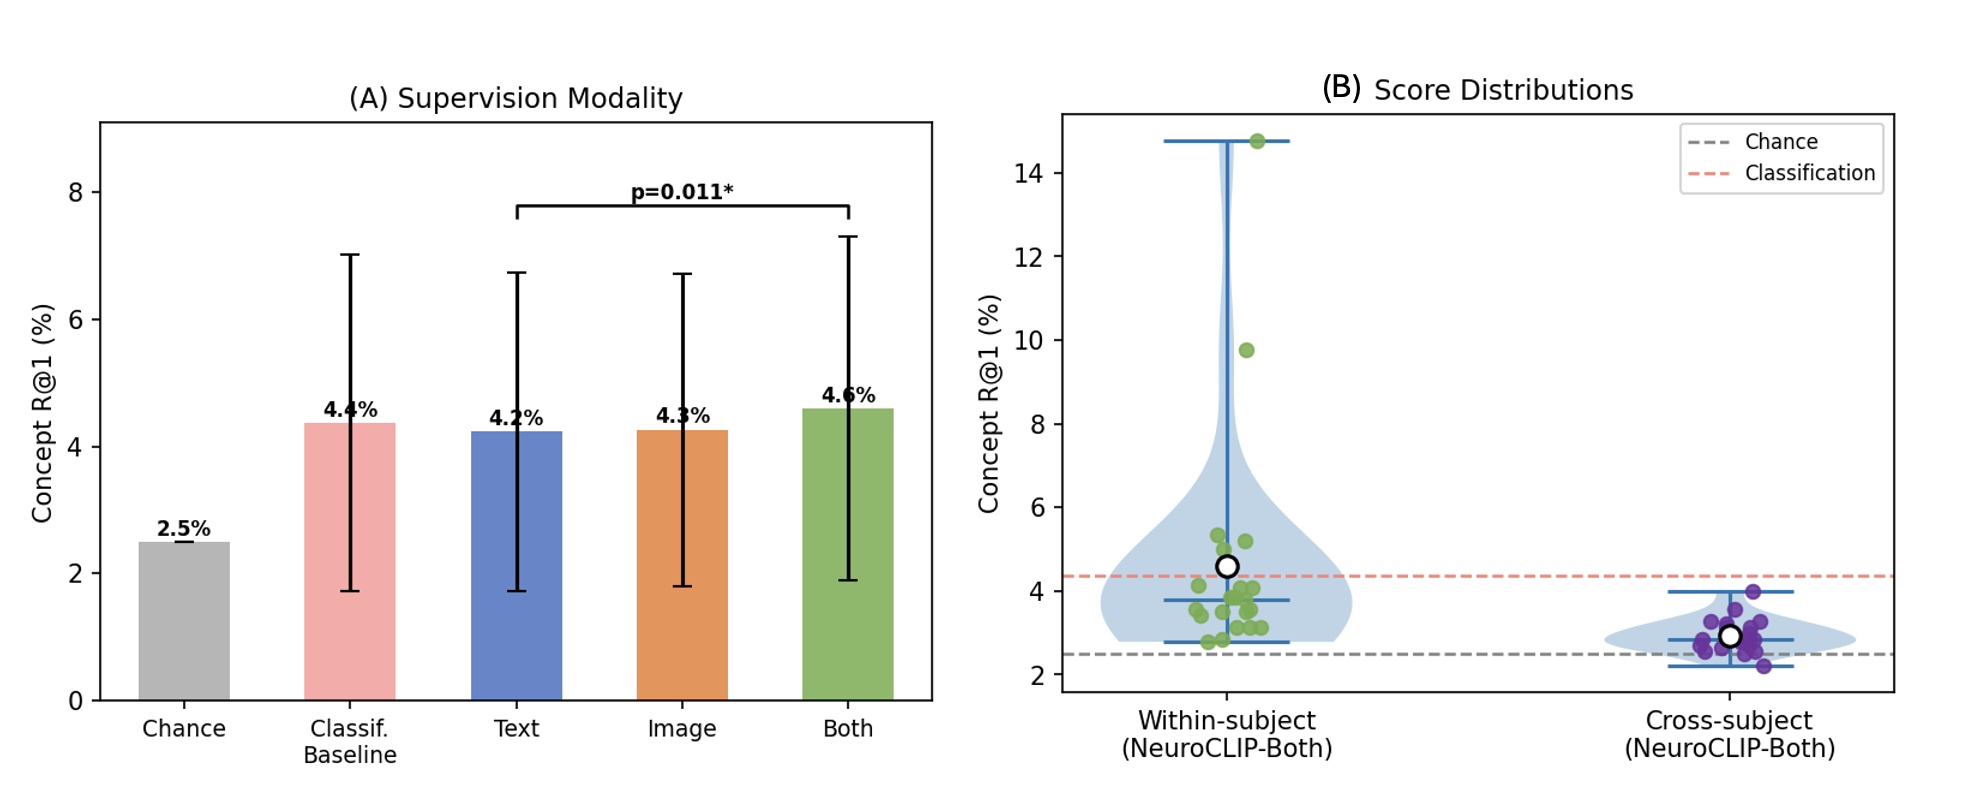
\includegraphics[width=0.78\linewidth]{figures/neuroclip_summary.png}
    \caption{NeuroCLIP summary diagnostics. EEG embeddings are trained to
    retrieve frozen CLIP concept targets instead of learned classifier weights.
    The summary panels compare supervised classification, text-only CLIP,
    image-only CLIP, and fused text+image targets against the 2.5\% chance
    level. Error bars show subject-recording variability; the fused target gives
    the best concept Recall@1 (4.60\%) while preserving a retrieval geometry
    that can be analyzed concept by concept.}
    \label{fig:neuroclip_overview}
\end{figure}

\subsection{LATA: Latency-Aware Temporal Alignment}

NeuroCLIP is concept-level: it asks what semantic information survives in EEG.
LATA addresses the complementary temporal question. A 2-second EEG clip and its
paired video are partitioned into $K$ chunks:
$\mathbf{E}=[\mathbf{e}_1,\ldots,\mathbf{e}_K] \in \mathbb{R}^{K \times d}$ and
$\mathbf{V}=[\mathbf{v}_1,\ldots,\mathbf{v}_K] \in \mathbb{R}^{K \times d}$.
Because neural responses lag the stimulus, chunk $\mathbf{e}_k$ may reflect
video evidence from $\mathbf{v}_{k-\delta}$ rather than $\mathbf{v}_k$. LATA
therefore maintains trainable logits $\boldsymbol{\ell} \in \mathbb{R}^{\Delta+1}$
over candidate delays:
\begin{equation}
    \mathbf{w} = \mathrm{softmax}(\boldsymbol{\ell}), \qquad
    \sum_{\delta=0}^{\Delta} w_\delta = 1.
\end{equation}
The latency-corrected video representation at chunk $k$ is
\begin{equation}
    \tilde{\mathbf{v}}_k
    =
    \sum_{\delta=0}^{\Delta} w_\delta \mathbf{v}_{k-\delta},
    \qquad
    \mathbf{v}_{k-\delta}=\mathbf{0}\ \mathrm{if}\ k<\delta.
\end{equation}
The corrected video sequence $\tilde{\mathbf{V}}$ is then used as keys and
values in cross-attention with EEG queries:
\begin{equation}
    \mathrm{LATA}(\mathbf{E},\mathbf{V})
    =
    \mathrm{MultiHeadAttn}(
    \mathbf{Q}=W_q\mathbf{E},
    \mathbf{K}=W_k\tilde{\mathbf{V}},
    \mathbf{V}=W_v\tilde{\mathbf{V}}).
\end{equation}

We optimize the EEG and video chunk embeddings with an InfoNCE objective:
\begin{equation}
    \mathcal{L}_{\mathrm{LATA}}
    =
    -\frac{1}{BK}\sum_{i=1}^{BK}
      \log
      \frac{
        \exp(\mathrm{sim}(\mathbf{n}_i,\tilde{\mathbf{v}}_i)/\tau)}
      {\sum_{j=1}^{BK}
        \exp(\mathrm{sim}(\mathbf{n}_i,\tilde{\mathbf{v}}_j)/\tau)}.
\end{equation}
Gradients flow through $\mathbf{w}=\mathrm{softmax}(\boldsymbol{\ell})$, so the
delay distribution is learned without any explicit delay labels. After training,
$\mathbb{E}[\delta]=\sum_\delta \delta w_\delta$ gives an interpretable estimate
of neural response delay in chunk units.

LATA is deliberately parameter-efficient: the only latency-specific parameter is the vector
$\boldsymbol{\ell}$, so any learned nonzero lag cannot be attributed to a large
delay-prediction subnetwork. The module can be inserted anywhere a standard
cross-attention layer would align paired temporal streams. In our experiments,
EEG chunks are encoded with a shallow temporal-spatial CNN, and video chunks are
represented by frozen CLIP frame embeddings sampled at matched chunk timestamps.
During training, LATA uses contrastive chunk matching to push each neural chunk
toward the latency-corrected visual chunk at the same index and away from other
chunks in the batch. During analysis, we inspect both the peak delay
$\delta^*=\arg\max_\delta w_\delta$ and the expected delay
$\mathbb{E}[\delta]$.

\FloatBarrier

% ============================================================
\section{Experimental Methodology}
% ============================================================

\paragraph{Dataset.}
We use SEED-DV~\citep{liu2024eeg2video}, which contains 62-channel EEG recorded
at 200\,Hz while subjects watched natural 2-second video clips. The benchmark
contains 40 concept categories, 5 clips per concept per block, and 7 session
blocks per subject. We evaluate raw EEG ($62 \times 400$), DE features, and PSD
features. DE and PSD compress each trial into 5 canonical frequency bands:
$\delta$, $\theta$, $\alpha$, $\beta$, and $\gamma$.

\paragraph{Splits and preprocessing.}
For supervised baselines and NeuroCLIP, we use within-subject leave-one-block-out
cross-validation: six blocks for training and one held-out block for testing,
rotated over the seven blocks. This prevents train/test session overlap. We use
train-only normalization statistics for leakage-controlled conditions and apply
them to validation/test folds. NeuroCLIP is evaluated on 21 subject-recording
files from the SEED-DV preprocessing artifacts, corresponding to the 20 subjects
plus one repeated subject recording used in the available files. LATA is run on
all 20 subjects with six train sessions and one held-out validation session.

\paragraph{Visual targets.}
For NeuroCLIP, we precompute frozen CLIP ViT-B/32 embeddings for concept labels
and/or representative visual frames. Concept-level galleries contain 40
normalized vectors, one per SEED-DV class. For LATA, video features are extracted
at the chunk level: each 2-second clip is divided into four 0.5-second chunks,
and one visual feature is assigned to each chunk. These frozen features ensure
that the trainable parameters are concentrated in the EEG encoder and the
alignment module, not in a large visual backbone.

\paragraph{Models and metrics.}
The supervised baseline uses the EEG2Video GLMNet-style feature classifier for
DE/PSD features and a raw-EEG-compatible encoder for raw signals. NeuroCLIP uses
the same within-subject fold structure but replaces the classifier with a CLIP
retrieval objective. We report Recall@1, Recall@5, Recall@10, mean reciprocal
rank (MRR), and per-concept retrieval. LATA uses $K{=}4$ chunks of 0.5\,s each,
$d_{\mathrm{model}}{=}128$, maximum delay $\Delta{=}3$, batch size 64, AdamW
with learning rate $3\times10^{-4}$, cosine annealing, and temperature
$\tau{=}0.07$. For LATA, the primary result is the learned delay distribution
rather than a classification accuracy gain.

\paragraph{Statistical analysis.}
We compare retrieval scores to chance using subject-level tests and report
concept-level analyses across the 40 classes. To test whether visual embedding
geometry explains EEG decodability, we correlate per-concept Recall@1 with CLIP
isolation and CLIP confusion. To test semantic effects, we compare activity
categories (sports, music, people) against passive categories. For protocol
validity, we report run-position accuracy profiles, session trends, and
within-concept prediction consistency against empirical random baselines.

\FloatBarrier

% ============================================================
\section{Results and Discussion}
% ============================================================

\subsection{Baseline and NeuroCLIP Retrieval Performance}

Table~\ref{tab:main_results} summarizes the main 40-way results. The supervised
DE baseline reaches 4.37\% top-1 and 17.17\% top-5 accuracy, above chance but
well below the originally reported EEG2Video GLMNet result. NeuroCLIP reaches
4.60\% concept Recall@1 and 17.47\% concept Recall@5 using CLIP text+image
targets. The absolute gain over the supervised DE classifier is modest; the main
benefit of NeuroCLIP is that retrieval exposes concept-level structure that a
single aggregate classification score cannot capture.

\begin{table}[!htbp]
\centering
\small
\setlength{\tabcolsep}{4pt}
\caption{Main 40-way concept results. Values are mean $\pm$ standard deviation
across subject-recordings for NeuroCLIP and across subjects for supervised
baselines. Chance is 2.5\% for top-1/R@1 and 12.5\% for top-5/R@5.}
\label{tab:main_results}
\begin{tabular}{>{\raggedright\arraybackslash}p{0.56\linewidth}cc}
\toprule
Condition & Top-1 / R@1 (\%) & Top-5 / R@5 (\%) \\
\midrule
Supervised DE baseline & $4.37 \pm 2.64$ & $17.17 \pm 5.44$ \\
Supervised DE, train-only normalization & $4.09 \pm 2.62$ & $16.84 \pm 5.19$ \\
Supervised PSD baseline & $4.15 \pm 2.60$ & $17.15 \pm 4.89$ \\
Supervised Raw EEG baseline & $3.79 \pm 1.56$ & $15.79 \pm 3.54$ \\
NeuroCLIP, DE $\rightarrow$ CLIP image & $4.26 \pm 2.46$ & $17.51 \pm 4.43$ \\
NeuroCLIP, DE $\rightarrow$ CLIP text+image & $\mathbf{4.60 \pm 2.70}$ & $\mathbf{17.47 \pm 5.14}$ \\
\midrule
Chance & $2.50$ & $12.50$ \\
\bottomrule
\end{tabular}
\end{table}

The ranked retrieval metrics show that the signal is not limited to exact top-1
hits. NeuroCLIP obtains R@1/R@5/R@10/R@20 of 4.57\%, 18.29\%, 32.98\%, and
58.0\%, respectively, and MRR of 0.143 versus a chance MRR of 0.107
($p=7.35\times10^{-5}$). These results indicate statistically reliable signal
despite the difficulty of 40-way EEG decoding from short natural videos.
Category-level retrieval is
also above chance: 15.5\% R@1 over 8 semantic categories versus 12.5\% chance,
and intra-category retrieval reaches 24.0\% versus 20.0\% chance.

Performance is highly subject dependent. Some recordings approach 10--15\%
R@1, while many are only slightly above chance. This subject variability is a
central practical limitation for EEG-based BCIs and explains why we use
within-subject models rather than a single pooled cross-subject model as the main
evaluation. It also motivates concept-level analysis: when aggregate accuracy is
low, a per-class probe can reveal whether the model is failing uniformly or
whether a subset of concepts carries most of the decodable signal.

The comparison between DE and raw EEG is also informative. Raw EEG preserves
the full 400-sample temporal waveform, but it underperforms the DE baseline in
the supervised setting and in NeuroCLIP-style retrieval. This does not imply
that temporal information is irrelevant; rather, it indicates that the current
raw encoder does not extract robust temporal features from the available amount
of subject-specific training data. The compressed DE representation may discard
within-clip dynamics, but it also averages over high-frequency noise and reduces
the dimensionality of the learning problem. This tradeoff motivates the two
directions we pursue: use DE features for stable concept-level semantic analysis,
and use LATA on chunked representations to study temporal alignment separately
from aggregate concept classification.

\subsection{Validity Checks: Leakage and Sequence Shortcuts}

Because SEED-DV uses concept-blocked presentation, we first checked whether
retrieval could be explained by simple protocol artifacts. Train-only
normalization did not produce a large collapse: DE top-1 changed from 4.37\% to
4.09\%, while PSD changed from 4.15\% to 4.29\%. This indicates that global
normalization was not the main source of above-chance performance, although
fold-level variance was affected and train-only normalization should be used for
future ablations.

We also stratified predictions by clip position within the 5-clip same-concept
run. DE accuracy across positions 1--5 was [4.40, 4.29, 4.48, 4.38, 4.10]\%,
and PSD was [3.84, 4.39, 4.29, 4.13, 4.31]\%. Neither profile shows a monotonic
run-position trend. Within-concept consistency is above random (DE: 24.3\% vs.
17.8\%), indicating that predictions are semantically structured, while the flat
run-position profile provides no evidence for a simple adaptation or anticipation
shortcut. These audits do not rule out every possible block-design artifact, but
they reduce the likelihood that the main results are driven by the most direct
sequence-position confound.

The remaining risk is block-level semantic priming: a subject sees five clips
from the same concept after a cue, so the EEG may contain concept expectation in
addition to stimulus-evoked visual processing. Our analyses partially address
this by using held-out session blocks and by showing no monotonic accuracy
profile across positions 1--5, but they cannot fully separate perceptual
evidence from concept-set maintenance. This distinction matters for deployment:
a BCI user would not normally experience a repeated concept cue immediately
before each decoded event. For this reason, we treat SEED-DV as a useful but
partly structured benchmark, and we emphasize relative comparisons and error
analysis over absolute claims about open-world decoding accuracy.

\subsection{What Predicts EEG Decodability?}

The most natural hypothesis is that EEG retrieval succeeds for concepts that are
well separated in CLIP space. This is not what we observe. Per-concept CLIP
isolation is essentially uncorrelated with NeuroCLIP Recall@1
($r=0.036$, $p=0.827$), and CLIP confusion is also uncorrelated with EEG
confusion (Spearman $\rho=-0.024$, $p=0.509$). In other words, NeuroCLIP is not
merely easier when the frozen gallery is geometrically convenient.

\begin{figure}[!htbp]
    \centering
    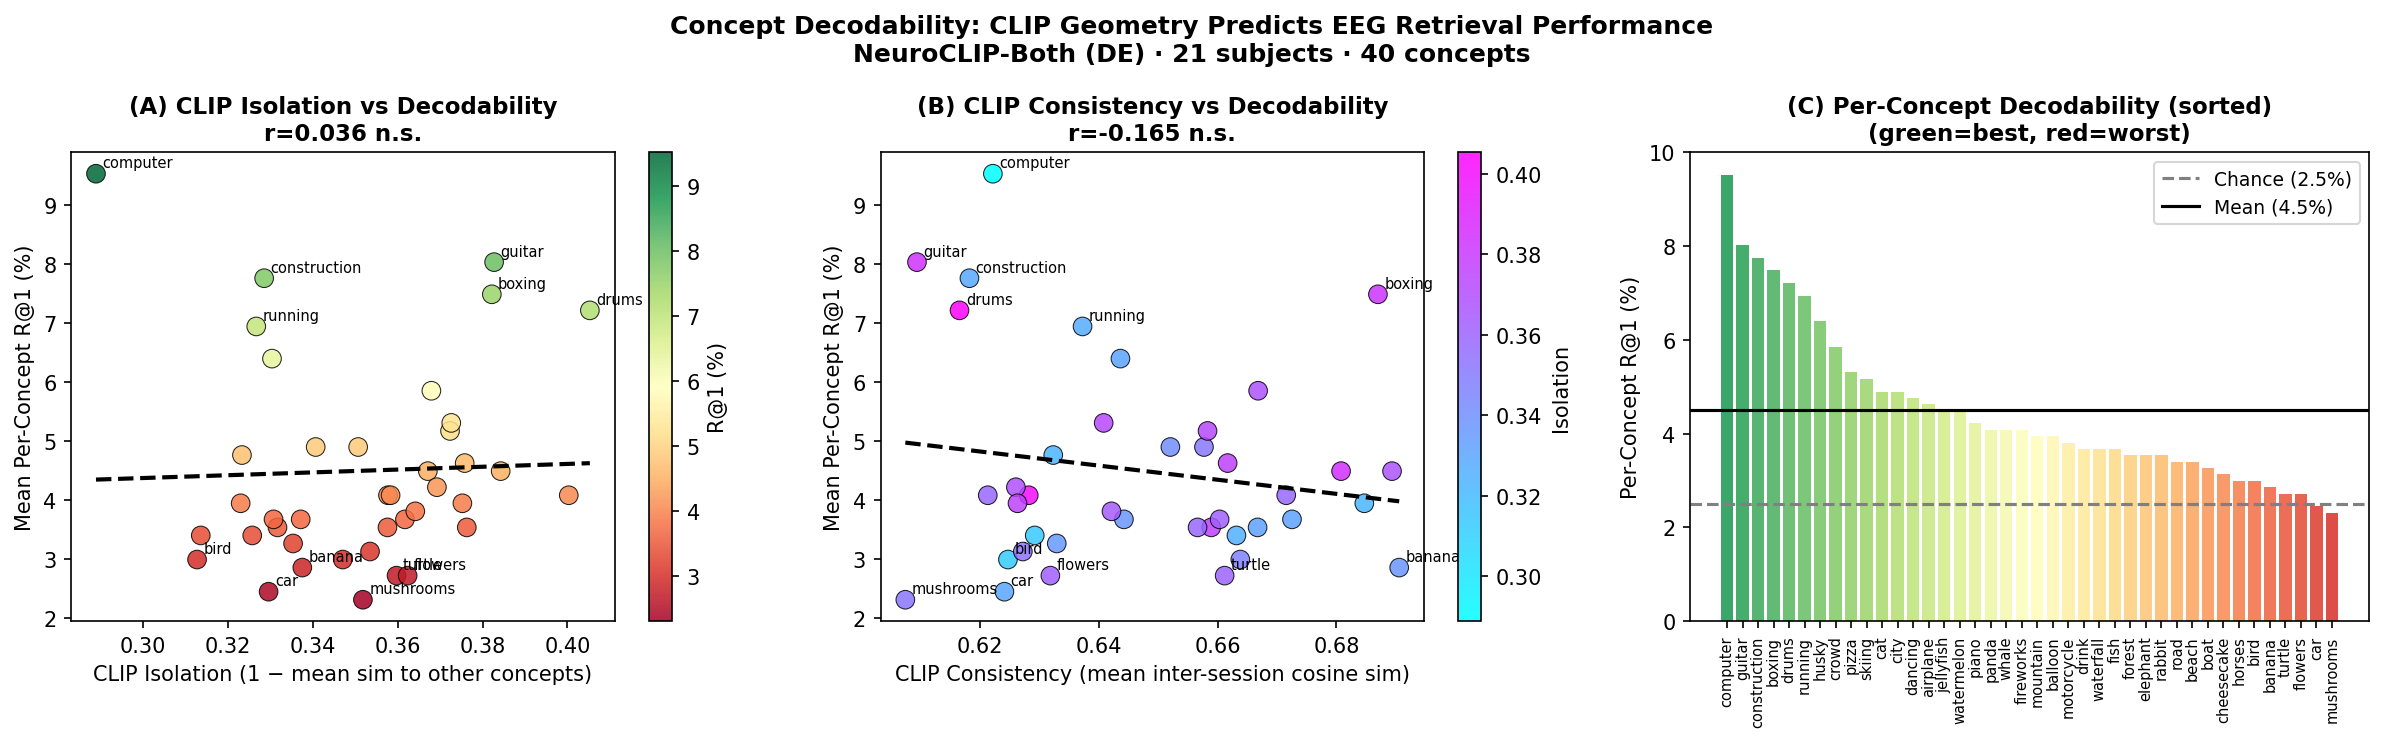
\includegraphics[width=0.90\linewidth]{figures/concept_decodability.png}
    \vspace{2pt}
    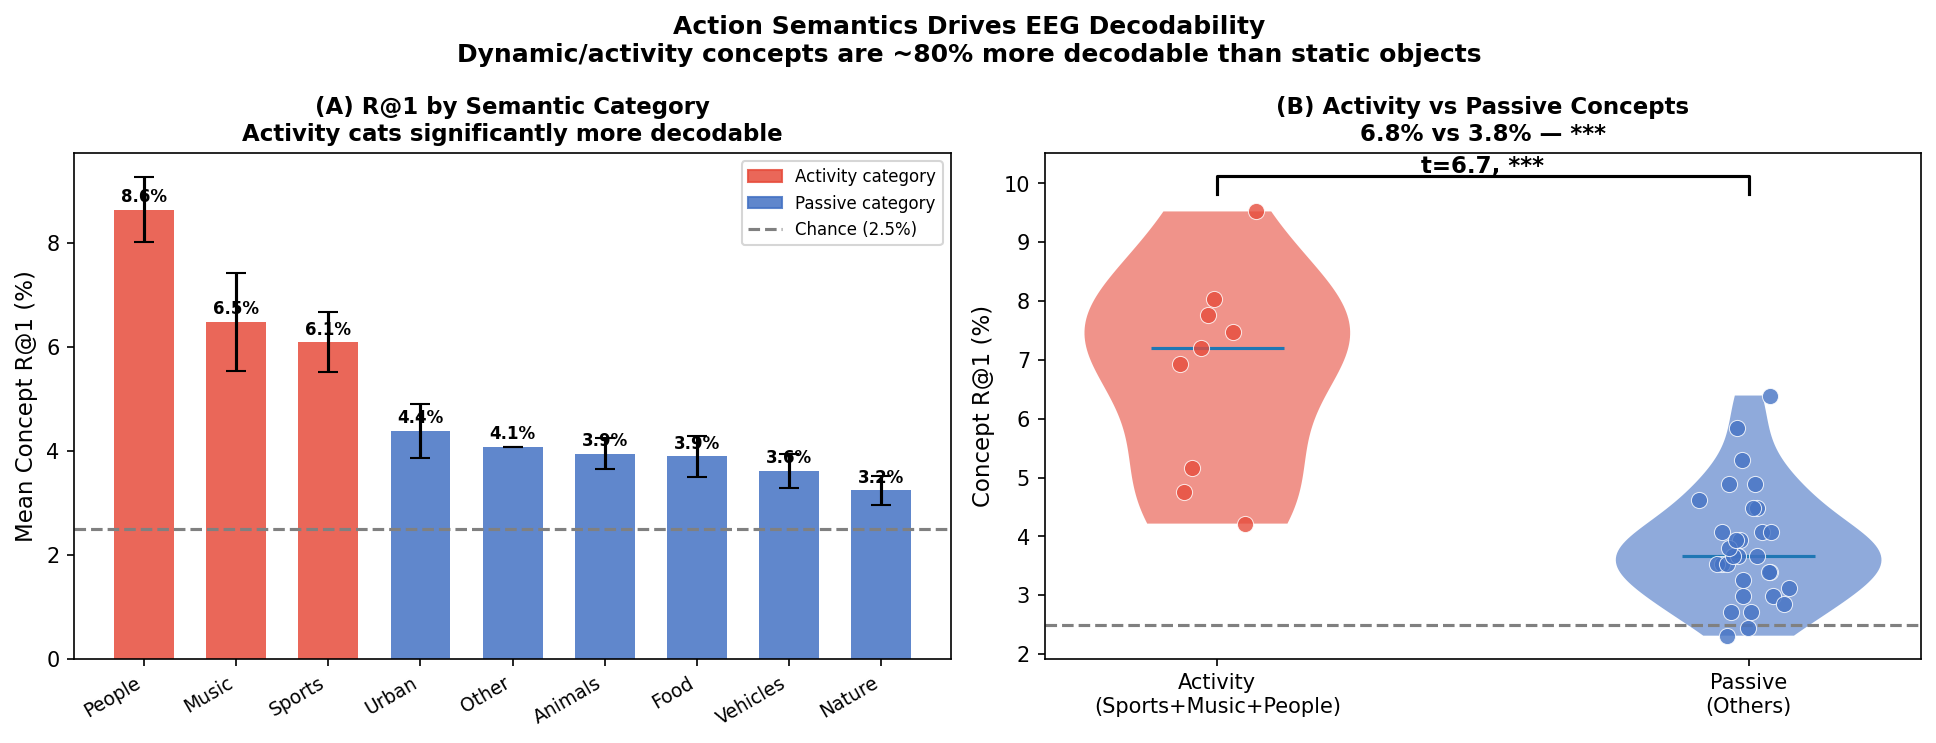
\includegraphics[width=0.90\linewidth]{figures/category_r1_analysis.png}
    \caption{NeuroCLIP concept-level error analysis. \textbf{Top:} concepts that
    are geometrically isolated in CLIP space are not systematically easier to
    decode from EEG: CLIP isolation has near-zero correlation with per-concept
    Recall@1 ($r=0.036$, $p=0.827$), and CLIP confusion does not match EEG
    confusion (Spearman $\rho=-0.024$, $p=0.509$). \textbf{Bottom:}
    decodability is instead structured by semantic content. Activity-rich
    concepts average 6.79\% Recall@1 versus 3.83\% for passive concepts
    ($t=6.72$, $p=5.95\times10^{-8}$), with a positive activity--passive gap in
    every session.}
    \label{fig:neuroclip_error}
\end{figure}

\FloatBarrier

The semantic category effect explains why aggregate accuracy is low but not
random: much of the recoverable signal is concentrated in a subset of concepts.
If evaluation is restricted to the top 10 most decodable concepts, R@1 rises to
6.97\%, compared with 4.50\% over all 40 concepts. Per-band DE comparisons show
no significant activity--passive difference across delta, theta, alpha, beta, or
gamma bands, suggesting that the advantage is not simply a global EEG power
effect.

The effect is also not a clean binary. Some non-action concepts, including
``computer'' and ``construction,'' rank highly, while some dynamic animal or
vehicle concepts rank lower. This points to a mixture of action, salience,
social content, object typicality, and within-concept visual consistency. A
useful follow-up would annotate each concept along these axes and model
per-concept EEG decodability as a multivariate response.

\subsection{LATA Learns a Consistent Nonzero Neural Lag}

LATA was first validated on paired synthetic sequences with known ground-truth
delays $\delta_{\mathrm{true}}\in\{0,1,2,3\}$, then applied to all 20 SEED-DV
subjects.

\begin{figure}[!htbp]
    \centering
    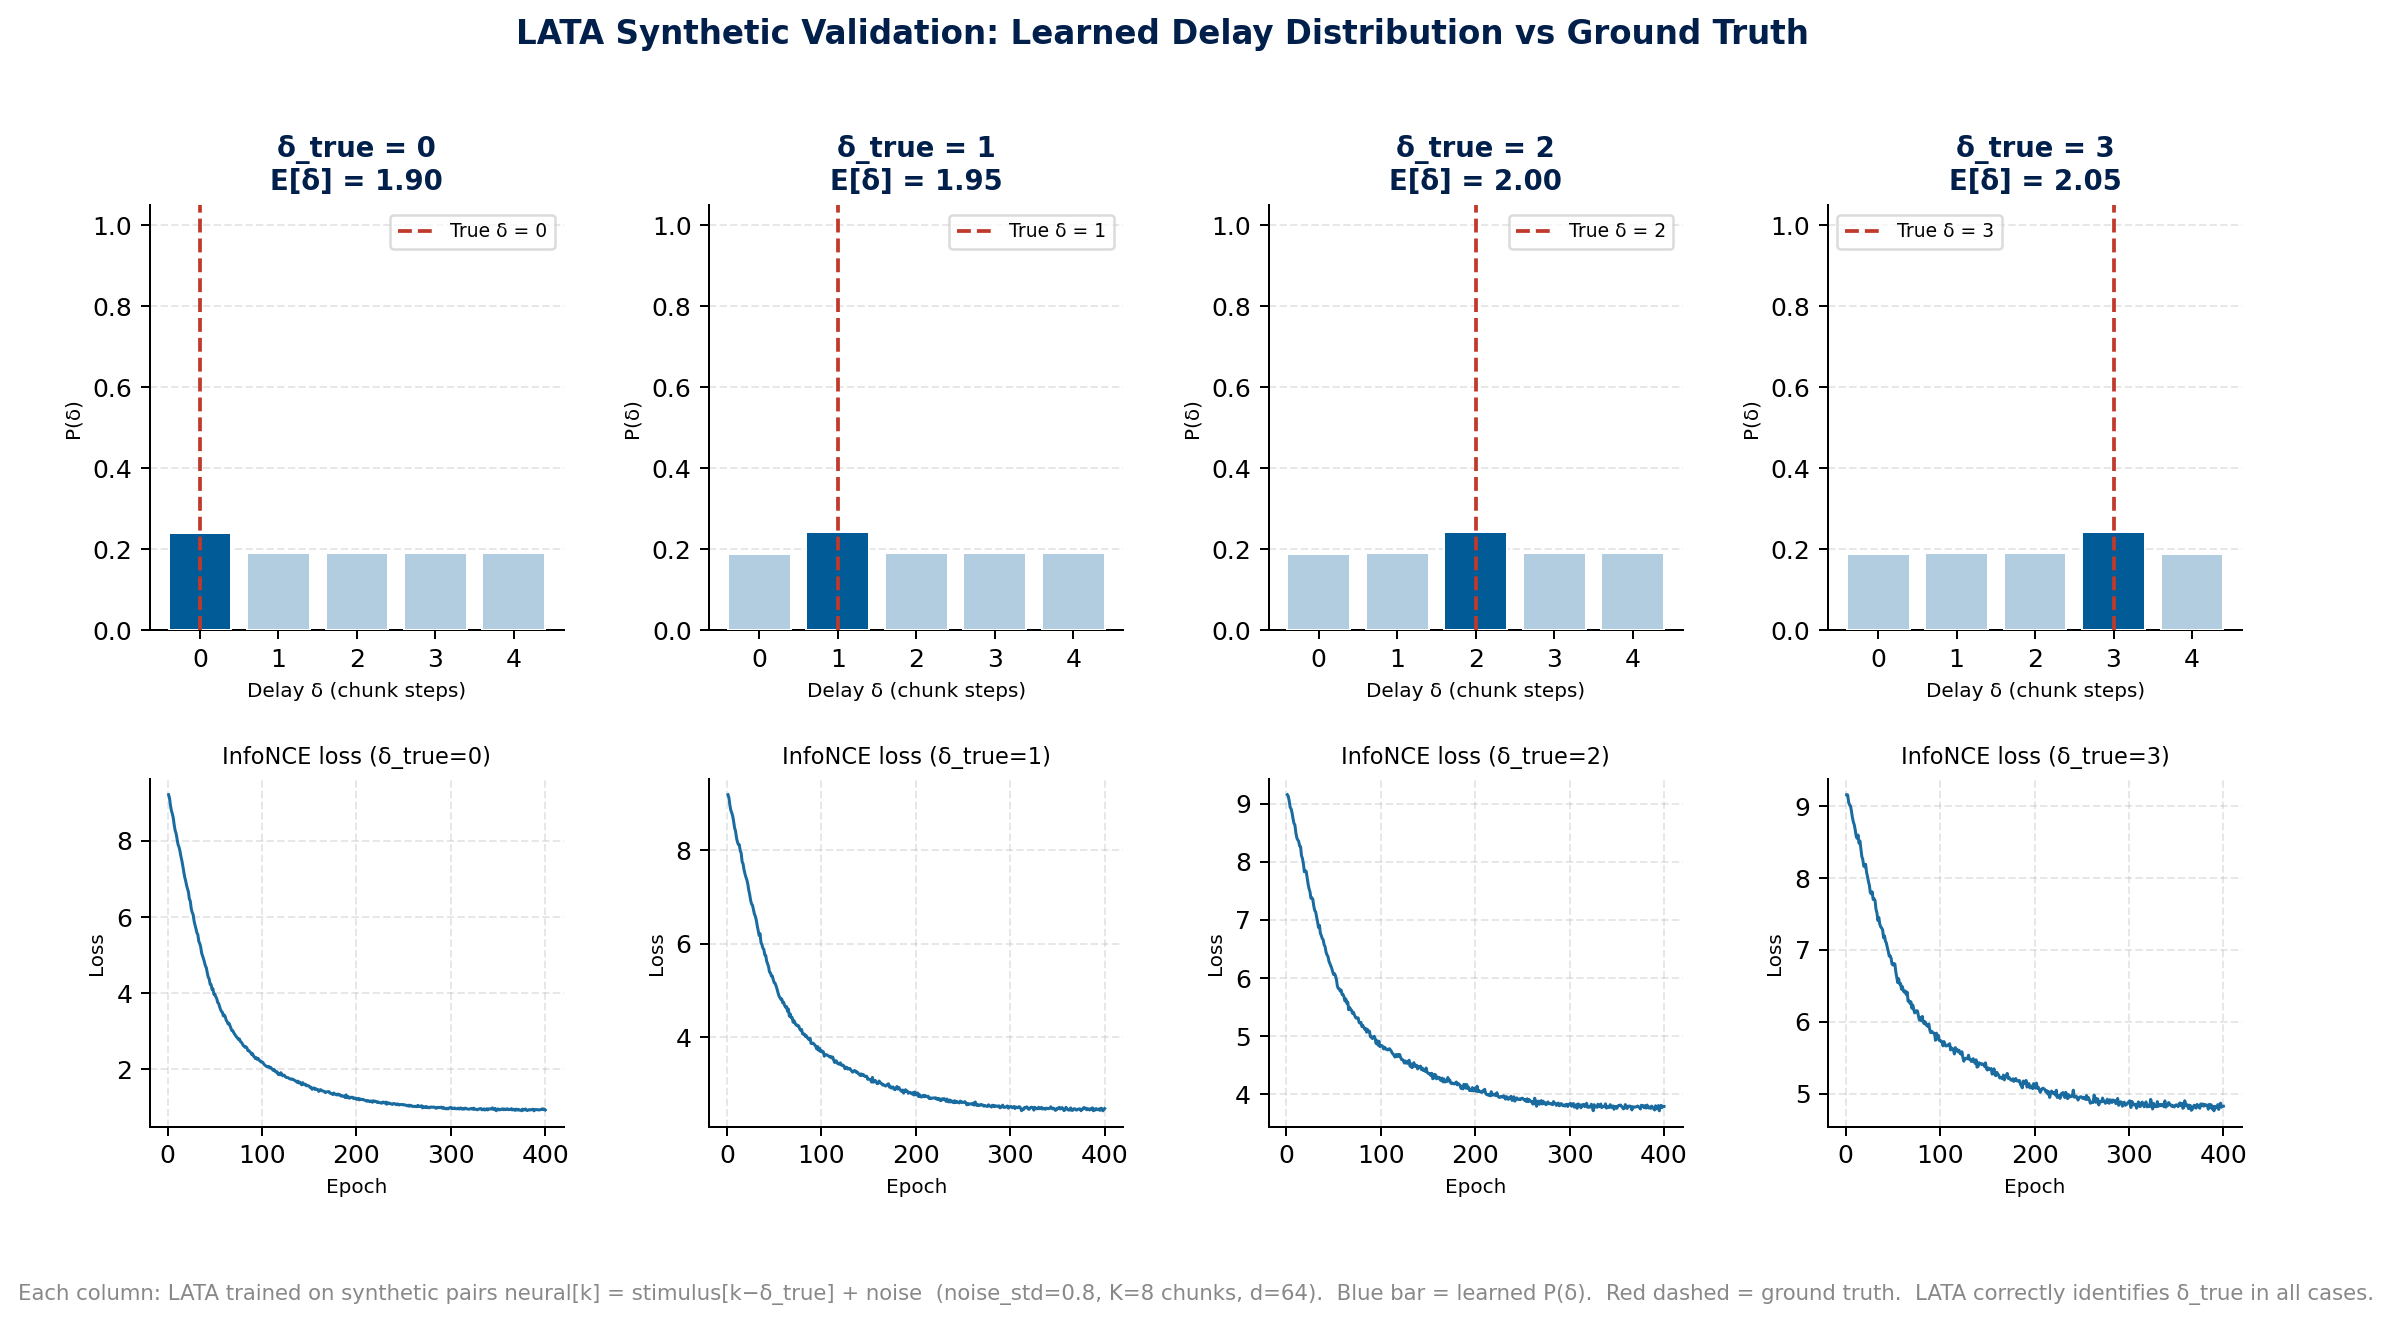
\includegraphics[width=0.76\linewidth]{figures/lata_synthetic_validation.png}
    \vspace{2pt}
    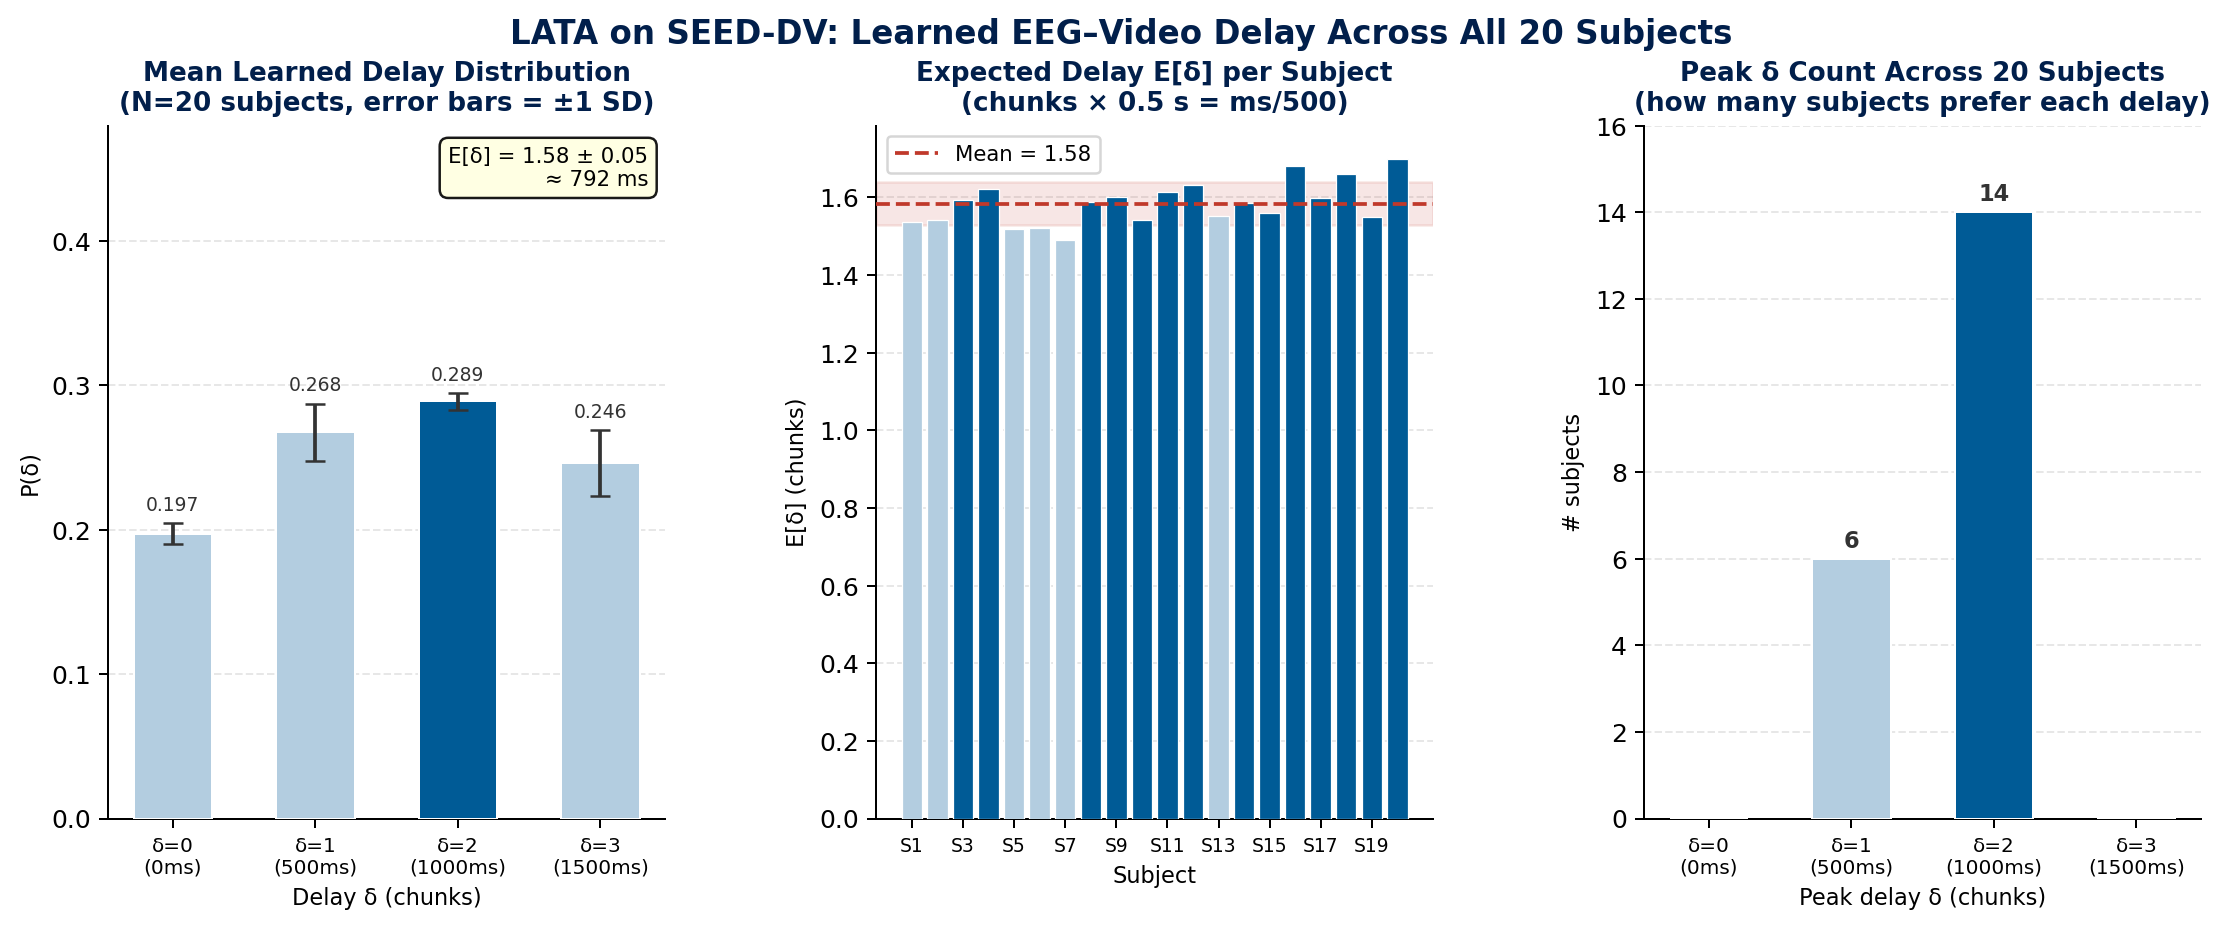
\includegraphics[width=0.76\linewidth]{figures/lata_all_subjects_results.png}
    \caption{LATA delay-learning results. \textbf{Top:} synthetic validation
    confirms that the differentiable delay distribution can recover known
    offsets $\delta_{\mathrm{true}}\in\{0,1,2,3\}$ from contrastive training
    alone. \textbf{Bottom:} on SEED-DV, learned delays are consistently nonzero:
    14/20 subjects peak at $\delta^*=2$, 6/20 peak at $\delta^*=1$, and no
    subject peaks at zero lag. The population mean distribution
    $[0.197,0.268,0.289,0.246]$ gives expected delay $1.58\pm0.05$ chunks
    ($\approx$790\,ms), supporting latency-aware rather than synchronous
    EEG--video alignment.}
    \label{fig:lata_results}
\end{figure}

On real EEG, LATA provides stronger evidence for interpretable latency
estimation than for improved held-out retrieval. The learned nonzero delay is
later than early visual components and is more consistent with semantic or late
positive processing, but $K=4$ chunks gives only coarse 500\,ms resolution. The
$\delta=2$ peak should therefore be read as evidence for delayed stimulus
evidence, not as a precise 1000\,ms ERP component.

Thus, LATA is best understood as an alignment diagnostic rather than a finished
retrieval model. It does not yet solve chunk-level EEG-video retrieval, but it
provides evidence against the zero-lag assumption used by many simple alignment
pipelines. The remaining softness of the learned distribution may reflect coarse
chunking, noise in CLIP frame features, or semantic processing distributed
across multiple late ERP components.

The latency result also clarifies why whole-clip concept retrieval and
chunk-level temporal alignment should be evaluated separately. A whole-clip
embedding can succeed by averaging delayed neural evidence over the full
2-second window; it does not need to know which video moment produced which EEG
response. LATA, by contrast, explicitly tests whether the model can align local
neural and visual events. Its current behavior indicates that coarse temporal
delay is learnable, but that fine-grained chunk retrieval remains substantially
harder than concept retrieval. This gap is an important negative result: dynamic
tracking cannot be assumed from above-chance whole-clip classification alone.

% ============================================================
\section{Conclusion and Future Work}
% ============================================================

This project studied EEG-to-video decoding through the lens of semantic and temporal interpretability. NeuroCLIP showed that 40-way EEG concept retrieval is above chance and comparable in scale to supervised EEG2Video-style classification, but its main value is diagnostic: CLIP geometry does not explain which concepts are decodable, while action-rich semantic content does. LATA addressed the temporal side of the same problem by learning neural response delay end-to-end. Across 20 subjects, the learned distributions consistently avoid zero lag and concentrate around one to two 0.5-second chunks.

Together, these findings refine how SEED-DV results should be interpreted. Above-chance concept accuracy is not uniformly distributed across the stimulus set, nor is EEG evidence temporally synchronous with the video stream. The benchmark contains meaningful neural signal, but that signal is selective and delayed. A model that improves average accuracy without examining these two factors may obscure the underlying structure of the decoding problem. Diagnostic tools such as NeuroCLIP and LATA instead identify where the signal is strongest and which alignment assumptions are least justified.

Several limitations remain. Absolute EEG decoding accuracy is low, and the largest NeuroCLIP gains are explanatory rather than performance-improving. The SEED-DV blocked design may contain subtler concept-priming or session-drift effects beyond what run-position stratification captures, and because SEED-DV concepts differ along correlated visual dimensions (motion, faces, object scale), the action advantage cannot yet be cleanly attributed to action semantics alone. LATA uses coarse 500 ms chunks and frozen CLIP frame features rather than spatiotemporal video encoders, so its latency estimates are approximate. Most importantly, both analyses are still within-dataset: they show structure in SEED-DV but do not yet prove that the same semantic and temporal patterns generalize.

Future work should evaluate NeuroCLIP on held-out concepts and additional EEG datasets
such as THINGS-EEG, where stimulus diversity is larger and block effects can be
tested more aggressively. For LATA, the next step is finer temporal resolution
(e.g., 100\,ms chunks), stronger frozen video encoders such as VideoMAE, and a
direct comparison between zero-lag cross-attention, fixed-lag alignment, and
learned-lag alignment. More broadly, our results support reporting concept-level
decodability, protocol audits, and learned temporal alignment diagnostics
alongside aggregate accuracy in EEG-to-video benchmarks.

The most important modeling extension is to unify the two diagnostics rather
than treating them as separate modules. A future \emph{Latency-Aware NeuroCLIP}
model would use LATA to compute latency-corrected EEG chunk embeddings, then map
those temporally aligned embeddings into the same CLIP concept space used by
NeuroCLIP. This addresses the natural next-step question: are the concepts that
NeuroCLIP finds decodable supported by specific delayed visual moments, or are
they only recoverable after averaging the whole 2-second EEG window? The unified
model would allow three concrete analyses: (i) compare whole-clip NeuroCLIP
retrieval against latency-corrected chunk-level retrieval; (ii) test whether
action-rich concepts remain easier because they contain stronger temporally
localized motion evidence; and (iii) estimate whether different semantic groups
prefer different delays, for example earlier motion and color responses versus later
object or concept responses. Ablations against zero-lag alignment, fixed-lag
alignment, and shuffled video chunks would distinguish genuine neural-video
correspondence from static category matching.

There are also smaller modeling extensions. NeuroCLIP could be trained with a
hierarchical objective that predicts coarse semantic category and fine concept
jointly, reducing the penalty for visually plausible confusions. LATA could be
made subject-adaptive by learning a population delay prior plus a small
subject-specific offset.

A final evaluation priority is moving beyond within-dataset validation. A
stronger benchmark would train on one subset of concepts and evaluate on held-out
concepts with matched semantic categories, or train on SEED-DV and evaluate on a
separate EEG vision dataset with different acquisition conditions. Such tests
would separate dataset-specific regularities from reusable neural-visual
correspondences.

\bibliographystyle{plainnat}
\bibliography{references}

\end{document}
